%%%%%%%%%%%%%%%%%%%%%%%%%%%%%%%%%%%%%%%%%%%%%%%%%%%%%%%%%%%%%%%%%%%%%%%%%%%%%%%%
%	TRABAJO: Proyecto Integrador
%		Titulo: 	Desarrollo de IP cores con procesamiento de Redes de Petri 	
%					Temporales para sistemas multicore en FPGA					
%		Autores:	Juli�n Nonino												%					Carlos Renzo Pisetta										%		Director:	Orlando Micolini											
%%%%%%%%%%%%%%%%%%%%%%%%%%%%%%%%%%%%%%%%%%%%%%%%%%%%%%%%%%%%%%%%%%%%%%%%%%%%%%%%

% Path im�genes: ./marco_teorico/FPGA_IP_HDL/img
% Nombre predeterminado im�genes: fpgaxx
%	xx es el numero de imagen

\chapter{FPGA - IP cores - HDL}
	\label{chap:chap_fpga_ip_hdl}
	
	El objetivo de esta secci�n, es introducir al lector en los conceptos de FPGA, IP core y HDL. Para ello, se comenzar� explicando brevemente qu� es una Field Programmable Gate Array (FPGA) y sus posibles usos. Luego, se continua con el concepto de IP Core, su clasificaci�n y algunos IP Cores que ser�n utilizados a lo largo de este trabajo. Para finalizar, se brindar� una introducci�n al lenguaje Verilog para que el lector adquiera las nociones b�sicas para entender la implementaci�n de este trabajo.

	% FPGA
		%%%%%%%%%%%%%%%%%%%%%%%%%%%%%%%%%%%%%%%%%%%%%%%%%%%%%%%%%%%%%%%%%%%%%%%%%%%%%%%%
%	TRABAJO: Proyecto Integrador
%		Titulo: 	Desarrollo de IP cores con procesamiento de Redes de Petri 	
%					Temporales para sistemas multicore en FPGA					
%		Autores:	Juli�n Nonino												%					Carlos Renzo Pisetta										%		Director:	Orlando Micolini											
%%%%%%%%%%%%%%%%%%%%%%%%%%%%%%%%%%%%%%%%%%%%%%%%%%%%%%%%%%%%%%%%%%%%%%%%%%%%%%%%

% Path im�genes: ./marco_teorico/FPGA_IP_HDL/img
% Nombre predeterminado im�genes: fpgaxx
%	xx es el numero de imagen

\section{Field Programmable Gate Array}
	\label{sec:fpga}

	Una FPGA (Field Programmable Gate Array) es un circuito integrado digital formado por bloques l�gicos los interconectados.

	Las interconexiones de una FPGA pueden ser conFigurados mediante un Lenguaje de Descripci�n de Hardware (HDL). De esta manera una FPGA puede reproducir desde simples compuertas l�gicas hasta complejos sistemas dentro de un solo chip.

	Existen FPGAs que pueden ser reprogramadas lo que les permite una gran flexibilidad a la hora de dise�ar circuitos digitales. Por otro lado, existen FPGAs que solo pueden programarse una �nica vez, su principal ventaja su menor consumo aunque al momento de dise�ar circuitos son mas complejas.

	En la \ref{fig:fpga01} se ve una FPGA dentro de una placa de desarrollo con diferentes perif�ricos ya conectados.
	
	Las caracter�sticas f�sicas a tener en cuenta en la elecci�n de una FPGA depender�n del proyecto que se desea emprender, pero, principalmente se consideran los siguientes puntos:
	\begin{itemize}
	  \item \emph{Cantidad de bloques l�gicos}: determina el espacio disponible para implementar la l�gica.
	  \item \emph{Tipo y tama�o de memoria}: pudiendo ser \emph{distribuida} o \emph{de bloques}, donde existe una memoria dedicada incluida en la FPGA o se utilizan los bloques l�gicos de la misma respectivamente.
	  \item \emph{Cantidad de puertos I/O}: usados como interface entre la FPGA y dispositivos externos.
	  \item \emph{Otros componentes internos}: Bloques de memoria, multiplicadores, PLL, CPU, conversores A/D, bloques DSP, etc.
	\end{itemize}
	
	\begin{raggedright}
	Las FPGA ofrecen las siguientes ventajas:
	\end{raggedright}	
	\begin{itemize}
		\item Gran flexibilidad de producto.
		\item Posibilidad de actualizar tanto el firmware como el hardware.
		\item Reutilizaci�n del hardware.
		\item Son dispositivos reconfigurables.
		\item Bajo costo respecto a los ASIC.
		\item Ejecuci�n de circuitos m�s r�pida que en otros dispositivos reprogramables.
		\item \textbf{La ejecuci�n de cada bloque se realiza concurrentemente, a diferencia de un micro controlador.}
		\item Gran utilidad para dise�o y testing de prototipos. 
	\end{itemize}
	\begin{raggedright}
		Por otro lado, tienen las siguientes desventajas:
	\end{raggedright}
	\begin{itemize}
		\item M�s costosas que los microprocesadores equivalentes.
		\item Mayor complejidad de dise�o (soft+hard).
		\item Retardos de propagaci�n mayores a los existentes en ASIC (Application Specific Integrated Circuit).
		\item Mayores costos en producci�n a gran escala.
		\item Consumo est�tico y din�mico moderados.
	\end{itemize}	
	\begin{figure}[H]
		\centering
		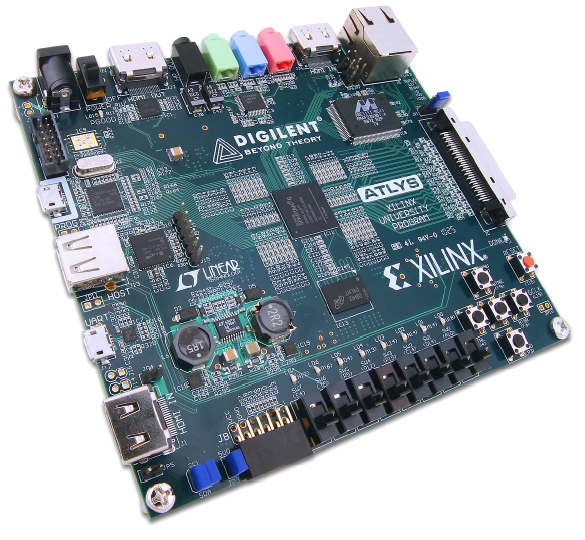
\includegraphics[width=.4\linewidth]{./marco_teorico/FPGA_IP_HDL/img/fpga01}
		\caption{Atlys Spartan-6 FPGA Development Board}
		\label{fig:fpga01}
	\end{figure}
	\newpage
		
	% IP cores
		%%%%%%%%%%%%%%%%%%%%%%%%%%%%%%%%%%%%%%%%%%%%%%%%%%%%%%%%%%%%%%%%%%%%%%%%%%%%%%%%%%%%%
%																					%
%	TRABAJO: Proyecto Integrador													%
%																					%
%		Titulo: 	Desarrollo de IP cores con procesamiento de Redes de Petri 		%
%					Temporales para sistemas multicore en FPGA						%
%																					%
%		Autores:	Juli�n Nonino													%
%					Carlos Renzo Pisetta											%
%		Director:	Orlando Micolini												%
%																					%
%	Parte: Marco Teorico															%
%	Capitulo: FPGA - IP cores - HDL													%
%	Seccion: Intellectual Property (IP) Core										%	
%	Archivo: ip_cores.tex															%
%																					%
%%%%%%%%%%%%%%%%%%%%%%%%%%%%%%%%%%%%%%%%%%%%%%%%%%%%%%%%%%%%%%%%%%%%%%%%%%%%%%%%%%%%%

% Path Imagenes: ./marco_teorico/FPGA_IP_HDL/img
% Nombre predeterminado imagenes: fpgaxx
%	xx es el numero de imagen


\section{Intellectual Property (IP) Core}
	\label{sec:ip_cores}

	Un \textbf{\emph{IP Core (Intellectual Property Core)}} es un bloque o m�dulo idealmente parametrizable 
	y reutilizable para usar en dise�os de FPGA o en ASIC. Posee una funcionalidad predefinida y es creado 
	con el uso de est�ndares, independizandolo de la herramienta de desarrollo.
	Los IP cores  se pueden licenciar en base a su funcionalidad. Existen dise�os de microprocesadores (soft-CPU) 
	o controladores de perif�ricos como USB, PCI, SDRAM, etc.
	
	Se puede clasificar un IP Core principalmente en tres categor�as:
	\begin{itemize}
	  \item \textbf{Hard Core:} Est�n dise�ados para una tecnolog�a espec�fica, tienen mejor 
	  		desempe�o y no pueden ser modificados por el dise�ador que los utiliza. Son poco 
	  		flexibles, portables y conFigurables pero son muy predecibles y fiables una vez 
	  		implementados. Tienen un layout predefinido incluido en la arquitectura.
	  \item \textbf{Firm Core:} Al igual que los \emph{hard}, incluyen informaci�n del mapeo a nivel 
	  		de compuertas y el c�digo fuente es visible para el dise�ador, haci�ndolos parcialmente 
	  		conFigurables. Suelen ser dise�ados y probados en diferentes tecnolog�as especificas, 
	  		ofreciendo una buena predictibilidad en cuanto a performance de tiempos de funcionamiento 
	  		y �rea utilizada, pero el usuario se ver� obligado a utilizar estos sobre las placas del 
	  		mismo fabricante.
	  \item \textbf{Soft Core:} Son los m�s flexibles y se distribuyen en c�digo de alto nivel HDL 
	  		permitiendo a los dise�adores modificarlo. Otro formato es mediante las netlist o lista 
	  		de compuertas e interconexiones. Ambos formatos los hace independientes de la tecnolog�a.
	\end{itemize}
	
	\begin{raggedright}
		\begin{tabular}{|p{2.5cm}||p{4cm}|p{4cm}|p{4cm}|}
			\hline
				& Hard Core & Firm Core & Soft Core\\
			\hline
			\hline
				Adaptabilidad & 
				Layout predefinido & 
				Mezcla de c�digo fuente y tecnolog�a dependiente de la netlist &	
				Dependiente del comportamiento del c�digo\\
			\hline
				Modelado & 
				Modelado como librer�a de elementos &
				Mezcla de bloques fijos y sintetizables que pueden ser compartidos por otros cores &
				Sintetizable con otra l�gica.\\
			\hline
				Flexibilidad & 
				No puede ser modificado por el dise�ador. Utilizar varios de �stos cores en un chip puede 
				resultar ineficiente. &
				Tecnolog�a dependiente.&
				El dise�o puede variarse.\\
			\hline
				Predictibilidad	&
				Garantiza los timing. &
				Camino critico es fijo. &
				Timing no garantizado.\\
			\hline
				Coste &	Bajo & Medio & Alto\\
			\hline
				Descripci�n &
				Ficheros layout y timing information. &
				C�digo sintetizable HDL y ficheros layout y timing information. &
				C�digo sintetizable HDL. \\
			\hline
		\end{tabular}
	\end{raggedright}
	\newpage
	Basados en estas caracter�sticas, se planteo desarrollar un \emph{Soft Core} debido a su gran 
	flexibilidad que permite futuras modificaciones.
		
	\subsection{MicroBlaze}
		
		El MicroBlaze \cite{xilinx_microblaze} es un procesador \emph{soft core} creado por Xilinx. Tiene 
		un set de instrucciones reducido (RISC) y esta optimizado para ser instanciado en una FPGA.
		\begin{figure}[H]
			\centering
			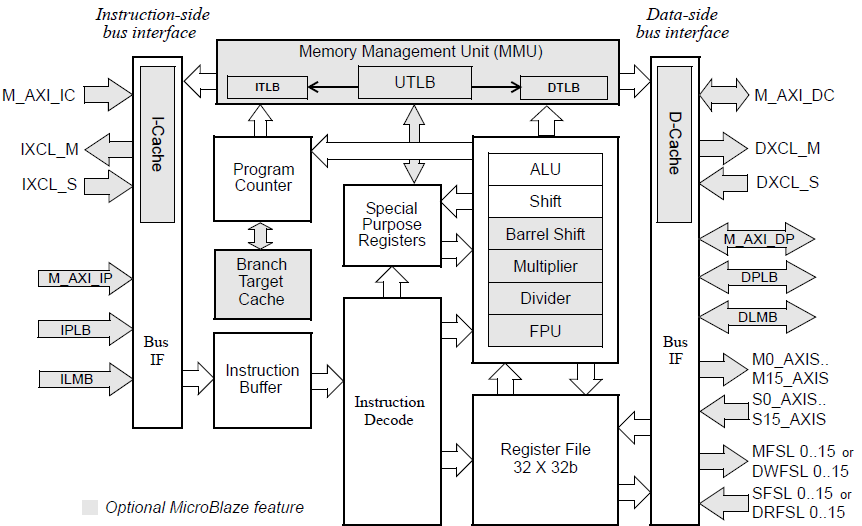
\includegraphics[width=0.9\linewidth]{./marco_teorico/FPGA_IP_HDL/img/fpga02}
			\caption{Diagrama en bloques de un core MicroBlaze}
			\label{fig:fpga02}
		\end{figure}
		
		\subsubsection{Caracter�sticas b�sicas}
			
			El MicroBlaze tiene las siguientes caracter�sticas fijas, es decir, no modificables.
			\begin{itemize}
			  	\item 32 de registros de 32 bits cada uno.
			  	\item Instrucciones de 32 bits con tres operandos y dos modos de direccionamiento.
			  	\item Bus de direcciones de 32 bits.
			\end{itemize}
			
			El resto de las caracter�sticas, pueden ser conFiguradas al momento de instanciarlo.
		
		\subsubsection{Endianismo}
			
			El MicroBlaze puede usar el formato Big-Endian o Little-Endian para representan los datos.
			La elecci�n depende del valor de un par�metro llamado: \emph{C\_ENDIANNESS}. 
			\\
			
			Los tipos de datos soportados por el procesador son:
			\begin{itemize}
			  	\item Word (32 bits).
			  	\item Half Word (16 bits).
			  	\item Byte (8 bits).  
			\end{itemize}
			 
		\subsubsection{Instrucciones}
			
			Las instrucciones del MicroBlaze se clasifican en dos tipos.
			\begin{itemize}
			  	\item \emph{Tipo A}: Toma dos operandos como fuente y uno como destino.
			  	\item \emph{Tipo B}: Toma un �nico operando como fuente, un operador inmediato de 16 
			  		bits y uno como registro destino. El operador de 16 bits puede ser convertido a 32 
			  		bits precediendo la instrucci�n tipo B con una instrucci�n ``Imm".
			\end{itemize}
		
		\subsubsection{Pipeline}
		
			El MicroBlaze ejecuta sus instrucciones de forma segmentada. Para la mayor�a de las instrucciones 
			cada etapa del pipeline toma un ciclo. Algunas pocas necesitan m�s de un ciclo en la etapa de 
			ejecuci�n, para	ello, se detiene el pipeline los ciclos necesarios.En general, se completa una 
			instrucci�n por ciclo.
			\\
			
			El pipeline del MicroBlaze puede ser de tres o cinco etapas dependiendo de la disponibilidad de 
			hardware que se tenga.
			\\
			
			Con el par�metro \emph{C\_AREA\_OPTIMIZED} en \emph{1} (uno), el pipeline se divide en tres etapas:
			\begin{enumerate}
			  	\item B�squeda de instrucci�n.
			  	\item Decodificaci�n de instrucci�n.
			  	\item Ejecuci�n de instrucci�n.
			\end{enumerate}
			
			
			Con el par�metro \emph{C\_AREA\_OPTIMIZED} en \emph{0} (cero), el pipeline se divide en cinco etapas:
			\begin{enumerate}
			  	\item B�squeda de instrucci�n.
			  	\item Decodificaci�n de instrucci�n.
			  	\item Ejecuci�n de instrucci�n.
			  	\item Accesos a memoria.
			  	\item Writeback.
			\end{enumerate}
		
		\newpage
		
		\subsubsection{Interfaces de conexi�n}
			
			El MicroBlaze soporta cuatro interfaces de conexi�n con perif�ricos: \emph{Local Memory Bus (LMB)},
			\emph{AMBA� AXI4 interface (AXI4)}, \emph{IMB Processor Local Bus (PLB)} y \emph{Xilinx CacheLink (XCL)}.
			
			El Local Memory Bus (LMB). Sirve para proveer acceso de un solo ciclo a una memoria block RAM 
			de dos puertos ubicada on-chip.
			
			Los buses AXI4 y PLB proveen conexiones a perif�ricos on-chip y off-chip adem�s de con la memoria.
			
			La interface CacheLink fue creada para usar con controladores de memoria externos.
			
			El MicroBlaze tambi�n soporta 16 puertos para interfaces Fast Simplex Link (FLS) o 4 AXI4-Stream. 
			Cada una con una interface master y una slave.
		
	\subsection{AXI}
	
		El \textbf{Advanced eXtensible Interface} (AXI) \cite{xilinx_axi} es un IP core que permite la 
		conexi�n entre IP cores. Puede tener hasta 16 IP cores de cada tipo conectados simult�neamente. Cada 
		uno puede usar anchos de datos de 32, 64, 128, 256, 512, 1024 independientemente del resto. El bus de 
		direcciones puede variar entre 12 y 64 bits.
	
		\subsubsection{Diagrama funcional}
		
			El \textbf{AXI Interconnect core} \ref{fig:fpga03} esta compuesto por dos interfaces, la interface 
			esclavo (slave), donde seconectan los dispositivos master y una interface maestro (master) donde se 
			conectan los dispositivos slave. Entre estas interfaces existen varias unidades funcionales divididas 
			en dos grupos, uno por cada Interface. En el medio se encuentra la crossbar encargada del ruteo de 
			peticiones entre los distintos dispositivos.
			\begin{figure}[H]
				\centering
				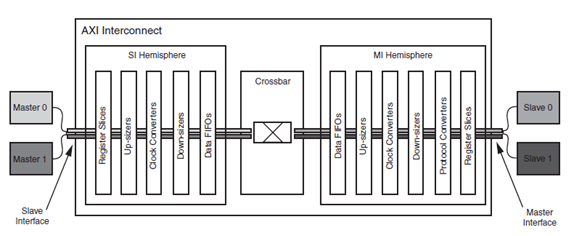
\includegraphics[width=0.95\linewidth]{./marco_teorico/FPGA_IP_HDL/img/fpga03}
				\caption{Diagrama de interconexi�n AXI}
				\label{fig:fpga03}
			\end{figure}
		\newpage
		\subsubsection{Tipos de conexi�n}
			El bus AXI permite la conexi�n entre IP cores master con los slave de las siguientes maneras:
			\begin{itemize}
			  	\item \textbf{Pass through}
			  		Este modo se utiliza cuando solo un master y un esclavo se conectan y no se utiliza ninguna 
					de las unidades funcionales de las que dispone el AXI.
			  		\begin{figure}[H]
						\centering
						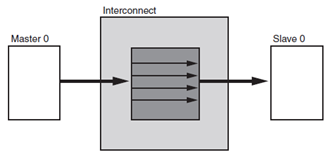
\includegraphics[width=.6\linewidth]{./marco_teorico/FPGA_IP_HDL/img/fpga04}
						\caption{Conexi�n AXI pass through}
						\label{fig:fpga04}
					\end{figure}
			  		
			  	\item \textbf{Conversion only}
			  		
			  		Este modo es conecta un master con un esclavo pero habilitando una o mas unidades funcionales 
					permitiendo conversi�n o funciones de pipeline. Las posibles unidades son:
					\begin{itemize}
						\item Conversi�n de tama�o de dato.
						\item Conversi�n de clock rate.
						\item Adaptaci�n de esclavo AXI4-Lite.
						\item Adaptaci�n de esclavo AXI-3.
						\item Pipelining, como registros de desplazamiento o canales de datos FIFO.
					\end{itemize}
					\begin{figure}[H]
						\centering
						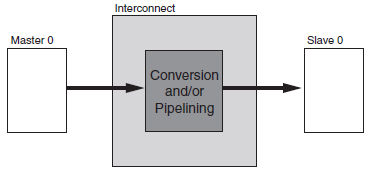
\includegraphics[width=.6\linewidth]{./marco_teorico/FPGA_IP_HDL/img/fpga05}
						\caption{Conexi�n AXI conversion only}
						\label{fig:fpga05}
					\end{figure}
			  	
			  	\item \textbf{N to 1 interconnect}
			  		
			  		Otro modo de usarlo es conectar m�ltiples masters a un �nico dispositivo esclavo. En este caso
					la decodificaci�n de direcciones es omitida salvo que la validaci�n de rango sea necesaria. En
					cualquier caso las conversiones de tama�o de dato o clock rate  pueden ser utilizadas.	
					\begin{figure}[H]
						\centering
						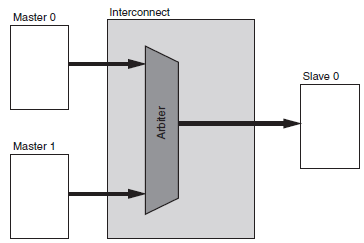
\includegraphics[width=.7\linewidth]{./marco_teorico/FPGA_IP_HDL/img/fpga06}
						\caption{Conexi�n AXI N to 1 interconnect}
						\label{fig:fpga06}
					\end{figure}
				
			  	\item \textbf{1 to N interconnect}
			
					Otro modo de uso valido es la conexi�n de un Master controlando varios esclavos. En este caso 
					el arbitraje de direcciones y escritura de datos no se realiza.
					\begin{figure}[H]
						\centering
						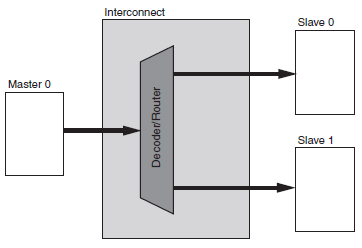
\includegraphics[width=.7\linewidth]{./marco_teorico/FPGA_IP_HDL/img/fpga07}
						\caption{Conexi�n AXI N to 1 interconnect}
						\label{fig:fpga07}
					\end{figure}
			  	
			  	\item \textbf{N to M interconnect (Crossbar)}
			
					En este modo se usa una topolog�a de direcci�n compartida y m�ltiples datos (SAMD). Consiste 
					en una crossbar para la escritura/lectura de datos y �rbitros para las direcciones.
					Existen caminos paralelos para escribir y leer por los cuales cualquier master puede acceder 
					a cualquier esclavo. Cuando m�s de una fuente accede a diferentes destinos se pueden realizar 
					estas operaciones de forma simult�nea.
					\begin{figure}[H]
						\centering
						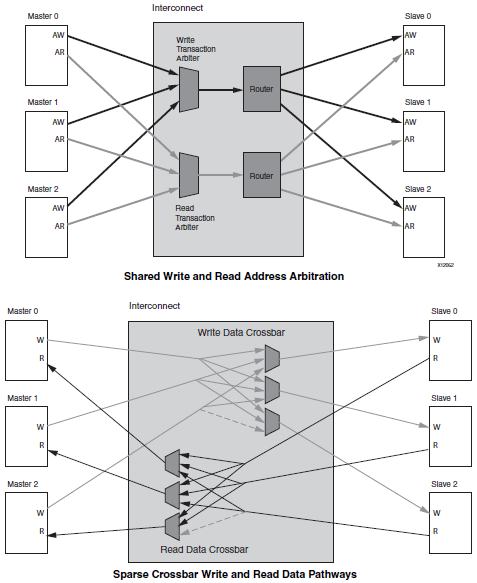
\includegraphics[width=0.8\linewidth]{./marco_teorico/FPGA_IP_HDL/img/fpga08}
						\caption{Conexi�n AXI N to M interconnect (Crossbar)}
						\label{fig:fpga08}
					\end{figure}
			  	
			  	\item \textbf{N to M interconnect (Shared Access)}
			
					En el modo compartido solo se puede realizar una transacci�n a la vez. Para cada master 
					conectado un pedido de lectura tiene prioridad sobre uno de escritura. El �rbitro selecciona 
					la solicitud a realizar entre las existentes. Este modo minimiza los recursos usados para 
					implementar el modulo de crossbar.
					\begin{figure}[H]
						\centering
						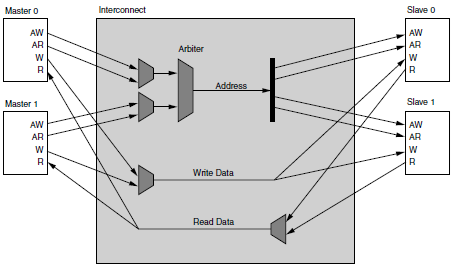
\includegraphics[width=.8\linewidth]{./marco_teorico/FPGA_IP_HDL/img/fpga09}
						\caption{Conexi�n AXI N to M interconnect (Shared Access)}
						\label{fig:Shared}
					\end{figure}	
			\end{itemize}
	
	
	% HDL
		%%%%%%%%%%%%%%%%%%%%%%%%%%%%%%%%%%%%%%%%%%%%%%%%%%%%%%%%%%%%%%%%%%%%%%%%%%%%%%%%%%%%%
%																					%
%	TRABAJO: Proyecto Integrador													%
%																					%
%		Titulo: 	Desarrollo de IP cores con procesamiento de Redes de Petri 		%
%					Temporales para sistemas multicore en FPGA						%
%																					%
%		Autores:	Juli�n Nonino													%
%					Carlos Renzo Pisetta											%
%					Orlando Micolini												%
%																					%
%	Parte: Marco Teorico															%
%	Capitulo: FPGA - IP cores - HDL													%
%	Seccion: Hardware Description Language (HDL)									%	
%	Archivo: hdl.tex																%
%																					%
%%%%%%%%%%%%%%%%%%%%%%%%%%%%%%%%%%%%%%%%%%%%%%%%%%%%%%%%%%%%%%%%%%%%%%%%%%%%%%%%%%%%%

% Path Imagenes: ./marco_teorico/FPGA_IP_HDL/img
% Nombre predeterminado imagenes: fpgaxx
%	xx es el numero de imagen

\lstset
{	language=Verilog,               % the language of the code
	basicstyle=\footnotesize,       % the size of the fonts that are used for the code
	numbers=left,                   % where to put the line-numbers
	numberstyle=\tiny\color{gray},  % the style that is used for the line-numbers
	stepnumber=1,                   % the step between two line-numbers. If it's 1, each line 
                       				% will be numbered
	numbersep=5pt,                  % how far the line-numbers are from the code
	backgroundcolor=\color{white},  % choose the background color. You must add \usepackage{color}
	showspaces=false,               % show spaces adding particular underscores
	showstringspaces=false,         % underline spaces within strings
	showtabs=false,                 % show tabs within strings adding particular underscores
	frame=none,                 	% adds a frame around the code
	rulecolor=\color{white},        % if not set, the frame-color may be changed on line-breaks within not-black text (e.g. comments (green here))
	tabsize=2,                      % sets default tabsize to 2 spaces
	captionpos=b,                   % sets the caption-position to bottom
	breaklines=true,                % sets automatic line breaking
	breakatwhitespace=false,        % sets if automatic breaks should only happen at whitespace
	%title=\lstname,                % show the filename of files included with \lstinputlisting;
		                            % also try caption instead of title
	keywordstyle=\color{blue},      % keyword style
  	commentstyle=\color{dkgreen},   % comment style
  	stringstyle=\color{mauve},      % string literal style
  	escapeinside={\%*}{*)},         % if you want to add LaTeX within your code
  	morekeywords={*,...},           % if you want to add more keywords to the set
  	deletekeywords={...}            % if you want to delete keywords from the given language
}

\section{Hardware Description Language (HDL)}
	\label{sec:hdl}

		Un lenguaje de descripci�n de hardware (HDL) permite definir las interconexiones y el comportamiento 
		de un circuito electr�nico y verificar el funcionamiento mediante simulaciones.
		 	
		\subsection{Verilog}
			
			Verilog \cite{ashenden}, es un HDL definido en un est�ndar de IEEE que soporta el dise�o, prueba e 
			implementaci�n de circuitos a diferentes niveles de abstracci�n. Su sintaxis es similar al del 
			lenguaje de programaci�n \emph{C}.

			\subsubsection{Verilog como lenguaje}
			
				El dise�o se describe como un conjunto de m�dulos. Utilizando la palabra clave \textbf{module}
				se define un m�dulo y se pueden especificar sus entradas y salidas y finalizan con una 
				sentencia endmodule como se muestra a continuaci�n:
				\begin{lstlisting}
module AOI (input A, B, C, D, output F)
	... descripci�n de funcionamiento ...
endmodule	
				\end{lstlisting}
				
			\begin{raggedright}
			Cada m�dulo es una unidad l�gica que incluye:
			\end{raggedright}
			\begin{itemize}
				\item Una interfaz para su conexi�n con otros m�dulos.
			  	\item Una descripci�n de su contenido mediante la especificaci�n de su comportamiento
			\end{itemize}
						
			El sentido de las conexiones con otros m�dulos puede ser de tres tipos, entradas (\emph{input}), 
			salidas (\emph{output}) o entrada-salida (\emph{inout}). Una vez que se ha definido el m�dulo se 
			puede instanciar cuantas veces sea necesario en el dise�o.
			
			Cada ejemplar del m�dulo que se utilice son elementos distintos por lo que se deben definir sus 
			conexiones con otros m�dulos.
			\\
			
			Verilog tiene b�sicamente dos tipos de datos. Por un lado, los \emph{par�metros}, estos, son constantes 
			definidas por el programador que no son implementadas en hardware pero ayudan a la descripci�n del
			comportamiento. 
			
			Por otro lado, las \emph{variables} y los \emph{registros}. Las variables se utilizan para 
			almacenar valores, pero esto no implica que se vean expl�citamente en la implementaci�n de hardware.
			
			Existen adem�s, los denominados \emph{wire} los cuales no retienen informaci�n, su funci�n es comunicar dos 
			o mas puntos de los cuales uno solo es el driver, es decir, el que puede modificar el estado 
			l�gico del cable.
			
			\subsubsection{L�gica de estados}
			
				Una variable en Verilog no solamente se representa con un $0$ y $1$, maneja una l�gica de cuatro 
				estados, los registros como wires pueden estar en uno de los siguientes:
				\begin{itemize}
					\item \textbf{X}: desconocido.
					\item \textbf{0}: false o nivel cero.
					\item \textbf{1}: true o nivel 1.
					\item \textbf{Z}: alta impedancia. 
				\end{itemize}
			
			\subsubsection{Buses}

				Los \emph{buses} o \emph{arrays} son elementos de varios bits que pueden ser del tipo \emph{wire} 
				o \emph{reg}. Los buses pueden ser usados como interfaz con otros m�dulos. A la hora de declararlos 
				se puede elegir la orientaci�n de los bits, es decir, \emph{MSB} el \emph{n} bit o \emph{MSB} el bit 
				\emph{0}, como se muestra en la Figura \ref{fig:fpga10}.
				\begin{figure}[H]
					\centering
					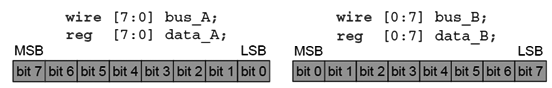
\includegraphics[width=.8\linewidth]{./marco_teorico/FPGA_IP_HDL/img/fpga10}
					\caption{Definici�n de buses en Verilog}
					\label{fig:fpga10}
				\end{figure}
				
				Las \emph{matrices} son un tipo de \emph{array de array} los cuales tienen la siguiente sintaxis de 
				definici�n.
				\begin{lstlisting}
reg [7:0] mem [0:3];
				\end{lstlisting}
				
				En ellas, se aplican las mismas definiciones de orden que para los array pero no pueden ser 
				usadas como interfaces con otros m�dulos.
			
			\subsubsection{Operadores}
				
				\begin{raggedright}
					\textbf{\emph{Operadores Binarios Aritm�ticos}}
				\end{raggedright}
				
				Existen cinco operadores aritm�ticos. Un detalle de su operaci�n es que si alg�n bit esta en 
				un estado desconocido el resultado tambi�n lo estar�.
				\begin{itemize}
				  	\item \textbf{\emph{+}} (\emph{suma o signo positivo}):
				  		Sirve para indicar una suma entre dos n�meros.
						\begin{lstlisting}
// B: 4'b1000   C: 4'b10
	A = B + C;
//Resultado A: 4'b1010
						\end{lstlisting}
				  	\item \textbf{\emph{-}} (\emph{resta o signo negativo}):
				  		Sirve para indicar la resta entre dos n�meros.
				  		\begin{lstlisting}
// B: 4'b1000   C: 4'b10
	A = B - C;
// Resultado A: 4'b0110
						\end{lstlisting}
				  	\item \textbf{\emph{*}} (\emph{multiplicaci�n}):
				  		Multiplica dos n�meros de cualquier tipo.
				  		\begin{lstlisting}
// B: 4'b0100   C: 4'b10
	A = B * C;
// Resultado A: 4'b1000
						\end{lstlisting}
				  	\item \textbf{\emph{/}} (\emph{divisi�n}):
				  		Divide dos n�meros de cualquier tipo.
				  		\begin{lstlisting}
// B: 4'b1000   C: 4'b10
	A = B / C;
// Resultado A: 4'b0100
						\end{lstlisting}
				  	\item \textbf{\emph{\%}} (\emph{resto}):
				  		Obtiene el resto de la divisi�n de dos n�meros de cualquier tipo.
				  		\begin{lstlisting}
// B: 4'b1000   C: 4'b10
	A = B \% C;
// Resultado A: 4'b0000
						\end{lstlisting}
				\end{itemize}

				\begin{raggedright}
					\textbf{\emph{Operadores de Igualdad}}
				\end{raggedright}
				
				Permiten comparar dos operandos, retornando $1$ � $0$, verdadero o falso respectivamente.
				\begin{itemize}
				  	\item \textbf{\emph{==, !=}} (\emph{igualdad}):
				  		El primero devuelve verdadero si los operando son iguales y falso en caso contrario. 
				  		El segundo indica desigualdad, funcionando al rev�s que el anterior. Si alg�n bit est� 
				  		en estado desconocido el resultado tambi�n lo estar�.
						\begin{lstlisting}
// A: 4'b1110   B: 4'b1101
	if (B != A)
//Resultado = true
						\end{lstlisting}
				  	\item \textbf{\emph{===, !==}} (\emph{igualdad}):
				  		Su funcionalidad es id�ntica a la anterior, pero difiere en tambi�n se comparan los valores 
				  		indefinidos ($X$) o de alta impedancia ($Z$).
				  		\begin{lstlisting}
// A: 4'b11X0   B: 4'b11X0
	if (B === A)
// Resultado = true
						\end{lstlisting}
				\end{itemize}				

				\begin{raggedright}
					\textbf{\emph{Operadores Relacionales}}
				\end{raggedright}
							
				Permiten comparar dos operandos, retornando $1$ � $0$, verdadero o falso respectivamente. Si 
				alg�n bit es $X$ el resultado tambi�n ser� $X$.
				
				\begin{itemize}
				  	\item \textbf{\emph{$>, \geq, <, \leq$}} (\emph{mayor, menor}):
				  		Poseen el significado habitual (mayor que, mayor o igual que, menor que, menor o igual que, 
						respectivamente).
						\begin{lstlisting}
// A: 4'b1110   B: 4'b1101
	if (B > A)
// Resultado = false
						\end{lstlisting}
				\end{itemize}
		
				\begin{raggedright}
					\textbf{\emph{Operadores L�gicos}}
				\end{raggedright}
				
				Aparecen entre dos operandos l�gicos y proporciona un valor l�gico (verdadero o falso).
				\begin{itemize}
				  	\item \textbf{\emph{!}} (\emph{negaci�n}):
				  		Cambia el valor l�gico del operando que va justo detr�s del operador.
				  		\begin{lstlisting}
// A = true
	if (!A)
// Resultado = false
						\end{lstlisting}
				  	\item \textbf{\emph{$\&\&$}} (\emph{AND l�gica}):
				  		El resultado ser� la combinaci�n de los dos operandos l�gicos. Es decir, para que 
				  		el valor sea verdadero, ambos operandos deben serlo, en caso contrario el resultado
				  		ser� falso.
				  		\begin{lstlisting}
// A = true ; B = false
	if (A && B)
// Resultado = false
						\end{lstlisting}
				  	\item \textbf{\emph{$\mid\mid$}} (\emph{OR logica}):
				  		El resultado ser� la combinaci�n de los dos operandos l�gicos. Para que el resultado sea 
				  		verdadero, bastar� con que uno de los operandos lo sea.
				  		\begin{lstlisting}
// A = true ; B = false
	if (A || B)
// Resultado = true
						\end{lstlisting}
				\end{itemize}

				\begin{raggedright}
					\textbf{\emph{Operadores L�gicos a nivel de bit}}
				\end{raggedright}
				
				Permite efectuar operaciones l�gicas con los bits de los operandos.	
				\begin{itemize}
					\item \textbf{\emph{$\sim$}} (\emph{negaci�n}):
				  		Negaci�n bit a bit.
				  		\begin{lstlisting}
// B: 4'b1110
	A = ~B;
// Resultado: A = 4'b0001
						\end{lstlisting}
					\item \textbf{\emph{$\&$}} (\emph{AND}):
						AND bit a bit.
						\begin{lstlisting}
// B: 4'b1110   C: 4'b1101
	A = B & C;
// Resultado: A = 4'b1100
						\end{lstlisting}
					\item \textbf{\emph{$\mid$}} (\emph{OR}):
						OR bit a bit.
						\begin{lstlisting}
// B: 4'b1110   C: 4'b1101
	A = B | C;
// Resultado: A = 4'b1111
						\end{lstlisting}
					\item \textbf{\emph{$\wedge$}} (\emph{XOR}):
						XOR bit a bit.
						\begin{lstlisting}
// B: 4'b1110   C: 4'b1101
	A = B ^ C;
// Resultado: A = 4'b0011
						\end{lstlisting}
					\item \textbf{\emph{$\sim\&$}} (\emph{NAND}):
						NAND bit a bit.
						\begin{lstlisting}
// B: 4'b1110   C: 4'b1101
	A = B ~& C;
// Resultado: A = 4'b0011
						\end{lstlisting}
					\item \textbf{\emph{$\sim\mid$}} (\emph{NOR}):
						NOR bit a bit.
						\begin{lstlisting}
// B: 4'b1110   C: 4'b1101
	A = B ~| C;
// Resultado: A = 4'b0000
						\end{lstlisting}
					\item \textbf{\emph{$\sim\wedge$}} (\emph{NOT XOR}):
						NOT XOR bit a bit. Tambi�n puede ser $\wedge\sim$.
						\begin{lstlisting}
// B: 4'b1110   C: 4'b1101
	A = B ~^ C;
// Resultado: A = 4'b1100
						\end{lstlisting}	
				\end{itemize}
				
				\begin{raggedright}
					\textbf{\emph{Operadores L�gicos de reducci�n}}
				\end{raggedright}
				
				El resultado de aplicar este operando al �nico argumento es un s�lo bit.	
				\begin{itemize}
				  	\item \textbf{\emph{$\&$}} (\emph{AND}):
						Se realiza un AND de todos los bits.
						\begin{lstlisting}
// B: 4'b1110
	A = &B;
// Resultado: A = 1'b0
						\end{lstlisting}
					\item \textbf{\emph{$\mid$}} (\emph{OR}):
						Se realiza un OR entre todos los bits del operando.
						\begin{lstlisting}
// B: 4'b1110
	A = |B;
// Resultado: A = 1'b1
						\end{lstlisting}
					\item \textbf{\emph{$\wedge$}} (\emph{XOR}):
						Se realiza un XOR entre todos los bits del operando.
						\begin{lstlisting}
// B: 4'b1110
	A = ^B;
// Resultado: A = 1'b1
						\end{lstlisting}
					\item \textbf{\emph{$\sim\&$}} (\emph{NAND}):
						Se realiza un NAND de todos los bits.
						\begin{lstlisting}
// B: 4'b1110
	A = ~&B;
// Resultado: A = 1'b1
						\end{lstlisting}
					\item \textbf{\emph{$\sim\mid$}} (\emph{NOR}):
						Se realiza un NOR entre todos los bits del operando.
						\begin{lstlisting}
// B: 4'b1110
	A = ~|B;
// Resultado: A = 1'b0
						\end{lstlisting}
					\item \textbf{\emph{$\sim\wedge$}} (\emph{NOT XOR}):
						Se realiza un NOT XOR entre todos los bits del operando. Tambi�n puede ser $\wedge\sim$.
						\begin{lstlisting}
// B: 4'b1110
	A = ~^B;
// Resultado: A = 1'b0
						\end{lstlisting}
				\end{itemize}
					  		
	  			\begin{raggedright}
					\textbf{\emph{Otros Operadores}}
				\end{raggedright}		
	  			
	  			\begin{itemize}
				  	\item \textbf{\emph{$\{,\}$}} (\emph{Concatenaci�n}):
				  		Concatenaci�n de dos operandos.
				  		\begin{lstlisting}
// B = 4'b0110  C = 4'b0010
	A = {B,C};  		// Resultado: A = 8'b01100010
	D = {2{B}}; 		// Resultado: D = 8'b01100110
	E = {B,C[1:0]}; // Resultado: E = 6'b011010}
						\end{lstlisting}
					
					\newpage	
						
				  	\item \textbf{\emph{$<<$}} (\emph{Desplazamiento izquierda}):
				  		Desplaza bits a la izquierda, a�adiendo ceros.
				  		\begin{lstlisting}
// A = 8'b11101101
	A << 2;  		
// Resultado: A = 8'b10110100
						\end{lstlisting}
				  	\item \textbf{\emph{$>>$}} (\emph{Desplazamiento derecha}):
				  		Desplaza bits a la derecha, a�adiendo ceros.
				  		\begin{lstlisting}
// A = 8'b11101101
	A >> 3;  		
// Resultado: A = 8'b00011101
						\end{lstlisting}
				  	\item \textbf{\emph{?}} (\emph{Condicional}):
				  		Dependiendo del resultado l�gico (verdadero o falso) se devolver� un valor u otro.
				  		\begin{lstlisting}
// A = 1'b1  B = 3'b111  C = 3'b001
	A == 1 ? B : C;	
// Resultado: A = 3'b111
						\end{lstlisting}
	  			\end{itemize}
	  			
			\subsubsection{Asignaciones}
				
				Existen dos tipos de asignaciones, por un lado est�n las bloqueantes las cuales se asemejan 
				a los cables simbolizadas con el $=$ como se muestra en la Figura \ref{fig:fpga11}.
					\begin{figure}[H]
						\centering
						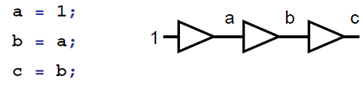
\includegraphics[width=.5\linewidth]{./marco_teorico/FPGA_IP_HDL/img/fpga11}
						\caption{Asignaci�n bloqueante en Verilog}
						\label{fig:fpga11}
					\end{figure}
				
				Por otro lado existen asignaciones anti bloqueantes o no bloqueantes. �stas asignaciones, se 
				sintetizan como \emph{latches} de manera tal que el ejemplo anterior se comporta como un 
				\emph{shift-register} (\ref{fig:fpga12}).			
					\begin{figure}[H]
						\centering
						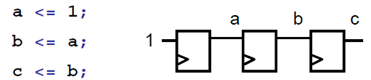
\includegraphics[width=.5\linewidth]{./marco_teorico/FPGA_IP_HDL/img/fpga12}
						\caption{Asignaciones NO bloqueantes en Verilog}
						\label{fig:fpga12}
					\end{figure}
				De esta manera el valor de \emph{c} tarda dos ciclos de reloj en tener el valor actual de \emph{a}.	
				
			\subsubsection{Procesos}
			
				\textbf{Uno de los aspectos m�s importantes en Verilog es la posibilidad de ejecutar en 
				paralelo varios procesos.}Cada proceso se ejecuta de forma secuencial, es decir se ejecuta 
				cada l�nea del proceso seg�n su orden de precedencia. Toda la descripci�n secuencial que se 
				quiera realizar en Verilog debe hacerse dentro de un proceso initial o always. La diferencia 
				entre ambos es que el primero se ejecuta una �nica vez y no es sintetizable, a diferencia del 
				always que se ejecuta cada vez que su lista de sensibilidad lo indique y si es sintetizable 
				en hardware.\\
				La lista de sensibilidad contiene todos los eventos por los que se debe ejecutar las 
				sentencias que contiene el proceso. A continuaci�n se muestra un ejemplo.
				\begin{lstlisting}
always@(/*lista de sensibilidad*/)
	begin
		/*Sentencias Secuenciales*/
	end
				\end{lstlisting}
							
			\subsubsection{Estructuras de Control}
				
				Verilog dispone de estructuras de control, similares a las disponibles en otros lenguajes de 
				programaci�n. Dentro de ellas las que pueden ser sintetizadas son las siguientes.
				\begin{itemize}
				  	\item \textbf{\emph{if - else}}:
				  		La sentencia condicional \emph{if-else} controla la ejecuci�n de otras. En caso de haber 
						m�ltiples sentencias es necesario hacer uso del bloque \emph{begin-end}. La sintaxis de 
						esta estructura es la siguiente.
				  		\begin{lstlisting}
if(/*expresion*/)
	begin
		/*Sentencias*/
	end
else
	begin
		/*Sentencias*/
	end
						\end{lstlisting}
					\item \textbf{\emph{Case}}:
				  		La sentencia \emph{case} es una instrucci�n de decisi�n m�ltiple, eval�a una expresi�n 
						y en funci�n de su valor ejecutar� las sentencias del caso correspondiente. Si existen 
						varias sentencias se debe usarse \emph{begin y end} para contenerlas. Si no se cubren 
						todos los posibles valores se debe hacer uso del caso por defecto, denominado 
						\emph{default}, el cual se ejecutar� cuando ninguno de los casos anteriores se cumpla. 
						La sintaxis de esta estructura es la siguiente.
				  		\begin{lstlisting}
case(/*expresion*/)
	caso 1:
		begin
			/*Sentencias*/
		end
	caso 2:
		begin
			/*Sentencias*/
		end
	.
	.
	.	
	default:
		begin
			/*Sentencias*/
		end		
endcase
						\end{lstlisting}
					\item \textbf{\emph{for}}:
				  		El bucle \emph{for} es id�ntico a los utilizados en otros lenguajes de programaci�n, 
						como en las estructuras mencionadas anteriormente, si existen varias sentencias se deben 
						incluir dentro del bloque \emph{begin-end}. Su sintaxis es la siguiente.
				  		\begin{lstlisting}
for(/*valor inicial*/ ; /*condicion de finalizacion*/ ; /*incremento*/)
	begin
		/*Sentencias*/
	end
						\end{lstlisting}	
				\end{itemize}
				